\chapter{Equipment Health Assessment using Artificial Neural Networks}
%\chapter{Classification of Healthy and Faulty States using Neural Networks}

\chapterintrobox{This chapter demonstrates the use of an artificial neural network to estimate the health state of a set of turbofan engines from NASA C-MAPSS dataset and predict the remaining useful life. Also different metrics to assess the performance of the network will be introduced.}

\section{Introduction to NASA C-MAPSS dataset}

C-MAPSS is a tool for simulating a realistic large commercial turbofan engine. The software is coded in the MATLAB\textsuperscript{\textregistered} and Simulink\textsuperscript{\textregistered} environment.

\begin{wrapfigure}{r}{0.5\textwidth}
    \centering
    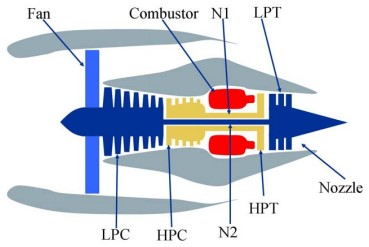
\includegraphics[width=.48\textwidth]{figures/c-mapss-engine-diagram.jpg}
    \caption{Simplified diagram of engine simulated in C-MAPSS \cite{Saxena2008}}
    \label{figure:c-mapss-engine-diagram}    
\end{wrapfigure}

It includes a number of editable input parameters that allow the user to enter specific values of his/her own choice regarding operational profile, closed-loop controllers, environmental conditions, etc. \cite{Saxena2008}. 

Figure \ref{figure:c-mapss-engine-diagram} is a simplified diagram of the simulated engine showing its main elements, like low pressure compressor section (LPC), high pressure compressor section (HPC), fan and combustor. The dataset released by NASA Ames Research Center contains resulting data from simulating many turbofine engines, from beginning of operation until failure. The dataset was originally released for Prognostics and Health Management 2008 Data Competition, Table \ref{table:c-mapss-sensors} shows different variables, the output of the simulation and their units, that were provided for the participants in the competition:

\begin{table}[ht]
    \centering
    \begin{tabu}{lll}
		\tabucline[1.5pt]{-} 
        \textbf{Symbol} & \textbf{Description} & \textbf{Units}\\
        \hline
        \textbf{T2} & Total temperature at fan inlet & R \\
        \textbf{T24} & Total temperature at LPC outlet & R \\
        \textbf{T30} & Total temperature at HPC outlet & R  \\
        \textbf{T50} &Total temperature at LPT & R\\
        \textbf{P2} & Pressure at fan inlet& psia\\
        \textbf{P15}& Total pressure in bypass-duct& psia\\
        \textbf{P30}& Total pressure at HPC outlet& psia\\
        \textbf{Nf}& Physical fan speed& rpm\\
        \textbf{Nc} & Physical core speed &rpm\\
        \textbf{epr}& Engine pressure ratio (P50/P2)& --\\
        \textbf{Ps30}& Static pressure at HPC outlet& psia\\
        \textbf{phi}& Ratio of fuel flow to Ps30& pps/psi\\
        \textbf{NRf}& Corrected fan speed &rpm\\
        \textbf{NRc}& Corrected core speed& rpm\\
        \textbf{BPR}& Bypass Ratio& --\\
        \textbf{farB}& Burner fuel-air ratio &--\\
        \textbf{htBleed}& Bleed Enthalpy &-- \\
        \textbf{Nf\_dmd} &Demanded fan speed& rpm\\
        \textbf{PCNfR\_dmd}& Demanded corrected fan speed &rpm\\
        \textbf{W31} & HPT coolant bleed & lbm/s \\
        \textbf{W32} & LPT coolant bleed & lbm/ \\
		\tabucline[1.5pt]{-} 
    \end{tabu}
    \caption{C-MAPSS outputs to measure system response.}
    \label{table:c-mapss-sensors}
\end{table}

C-MAPSS data contains 4 datasets: FD001, FD002, FD003 and FD004. Each dataset has different working conditions and fault modes. Table \ref{table:c-mapss-statistics} contains statistics of the different datasets:

\begin{table}[ht]
    \centering
    \begin{tabu}{ccccc}
        
		\tabucline[1.5pt]{2-5} 
                    & units number  & max length    & average length    & min length    \\
       \hline
            FD001   & 100           & 362           & 206.31            & 128           \\
            FD002   & 260           & 378           & 206.77            & 128           \\
            FD003   & 100           & 525           & 247.2             & 145           \\
            FD004   & 249           & 543           & 245.95            & 128           \\
		\tabucline[1.5pt]{-} 
    \end{tabu}
    \caption{Units number and cycles length statistics in C-MAPSS data}
    \label{table:c-mapss-statistics}
\end{table}

\section{Visualization of equipment degredation}
Visualizing the simulation output can give a sense of how these variables change during the life of the engine, Figure \ref{fig:sensors-plot} shows four different sensors from one of the engines (values are normalized):

\begin{figure}[h]
    \centering
    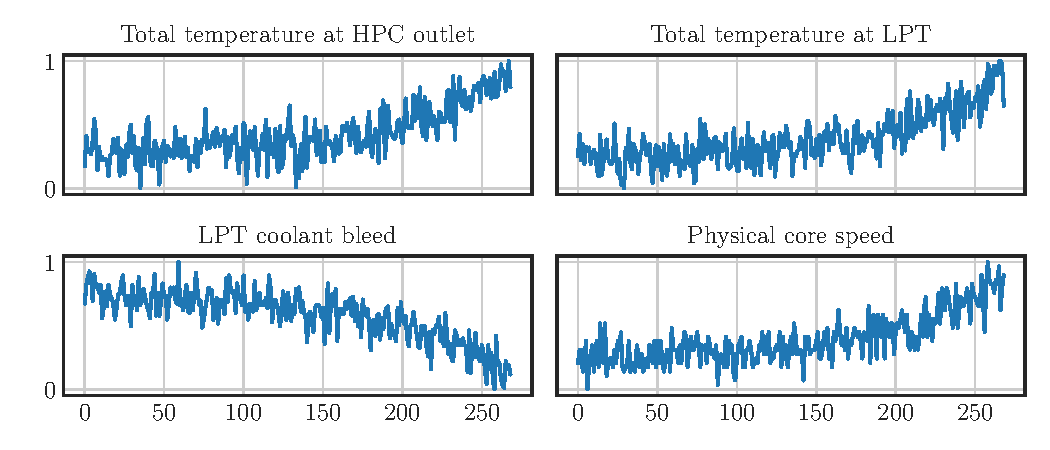
\includegraphics[width=\linewidth]{figures/plots/sensors_plot.pdf}
    \caption{Development of 6 sensors outputs from one of the engines (normalized)}
    \label{fig:sensors-plot}
\end{figure}
\begin{figure}[H]
    \centering
    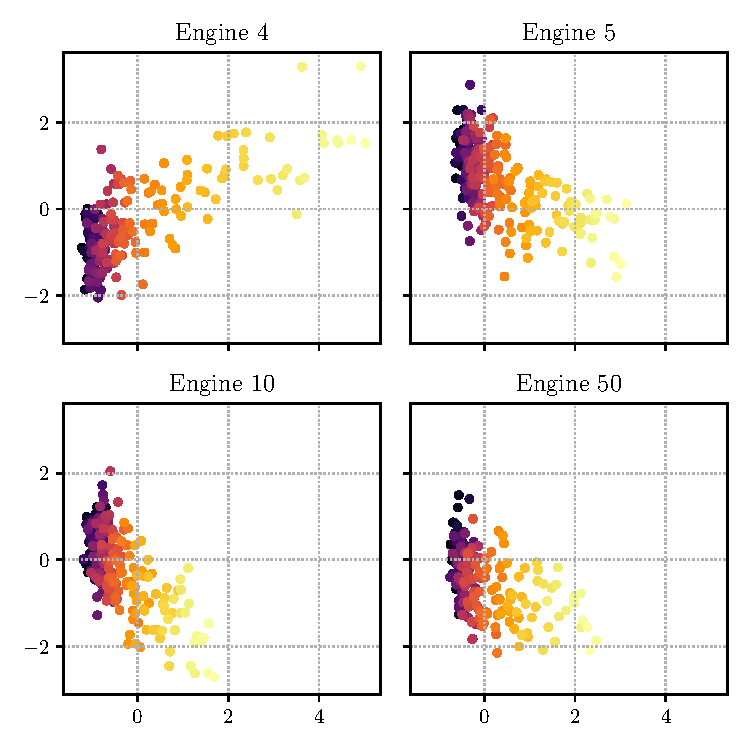
\includegraphics[width=.9\linewidth]{figures/plots/pca-degradation.pdf}
    \caption{Equipment health degredation (lighter colors indicate advancing of health degradation) of four turbofan engines from C-MAPSS dataset}
    \label{fig:pca-degradation}
\end{figure}

It is apparent that sensors output follow a specific pattern (increasing or decreasing) from beginning of operation until breakdown, this is very useful and can increase the robustness of the predictive model.

Alternatively, all sensors values can be combined and visualized altogether using Principal Component Analysis (section \ref{section:dimensionality-reduction}) to reveal the general trend in the data a dimsneionality reduction technique, if condition monitoring data is directly indicative of the equipment health state, visualization of principal components can show apparent visual degradation patterns.

Sensors values from 4 different engines are combined using PCA and the two first principal components are represented on Figure \ref{fig:pca-degradation}. 

There is absolutely an apparent pattern for health state degradation across the different engines from left (where darker colors indicate normal working state) to the right (where the lighter colors indicate fault development).

\section{Engines health classification}
Before proceeding with a complicated task such as RUL estimation, a simpler task like engines health classification can show the complexity of the problem. This section describes using neural networks to classify engines states as healty or faulty. The first and last 25 cycles from each unit are considered to be healthy and faulty respectively.

A neural network that uses all 24 inputs (all operational settings and sensors) with two hidden layers is used to carry out this classification. Table \ref{table:c-mapss-classifier-architecture} summarizes the network architecture:

\begin{table}[ht]
    \centering
    \begin{tabu}{lll}
		\tabucline[1.5pt]{-}
		\textbf{Layer (type)}   & \textbf{Output shape} &   \textbf{Param \#} \\
		\tabucline[1pt]{-}
		Dense1 (Dense) 			&   (None, 8)   &   200\\
		Dense2 (Dense) 	        &   (None, 4)   &   36       \\
		Dense3 (Dense)			&   (None, 1)   &   5   \\
		\tabucline[1pt]{-}
		Total params: 241       &                   &           \\
		Trainable params: 241   &                   &           \\
		Non-trainable params: 0     &                   &           \\
	\tabucline[1.5pt]{-}
    \end{tabu}
    \caption{C-MAPSS classifier architecture}
    \label{table:c-mapss-classifier-architecture}
\end{table}

The network is developed using Python and Keras framework \cite{chollet2015keras}.

The model is trained for 200 epochs with batch size of 32 samples, the classifier achieves \textbf{93.46\% accuracy} on the test set. Figure \ref{fig:cmapss-classifier-training} shows the training process of the network. The upper plot corresponds to the network loss where the x-axis shows training epochs and y-axis shows the train and validation losses (binary crossentropy). The lower plot corresponds to the network train and validation accuracies. Although the validation accuracy varies a lot, the training accuracy keeps improving with each epoch.

\begin{figure}[H]
    \centering
    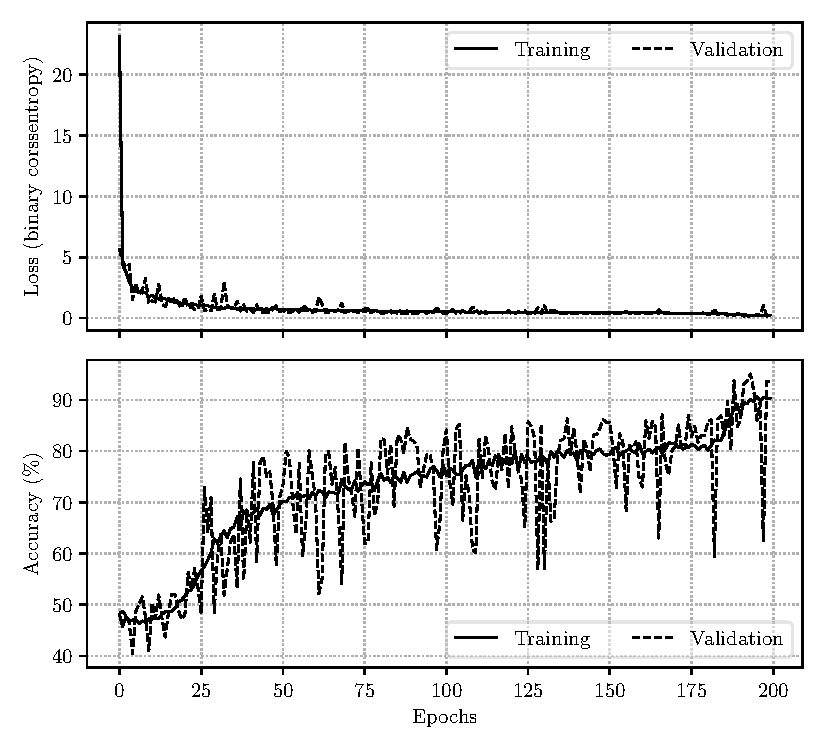
\includegraphics{figures/cmapss_classification_training.pdf}
    \caption{Training process of C-MAPSS classifier}
    \label{fig:cmapss-classifier-training}
\end{figure}

Figure \ref{fig:cmapss-classifier-roc} shows \acrlong{roc} (\acrshort{roc}) Curve of the classifier with a high \acrlong{auc} (\acrshort{auc}). Other classification metrics are shown in Table \ref{table:cmapss-classifier-metrics}.

\begin{figure}[H]
    \centering
    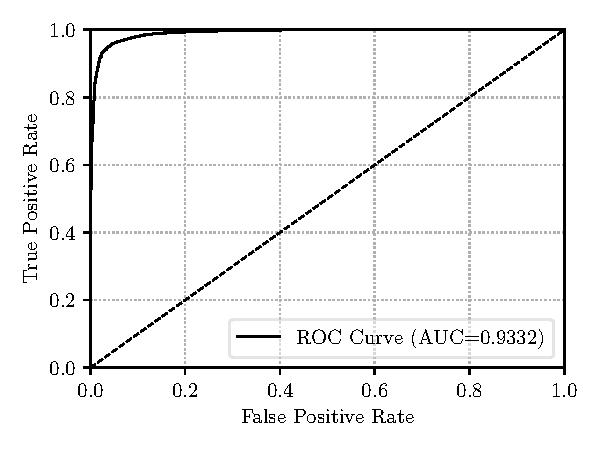
\includegraphics{figures/cmapss_classification_roc.pdf}
    \caption{C-MAPSS classifier ROC curve on test set}
    \label{fig:cmapss-classifier-roc}
\end{figure}

\begin{table}[H]
    \centering
    \begin{tabu}{cccccc}
        
    \tabucline[1.5pt]{-}
    \textbf{Metric} &  \textbf{Accuracy} &  \textbf{Precision} &  \textbf{Recall} &  \textbf{F-1} &  \textbf{ROC AUC}  \\
    \hline
    \textbf{Score} & 93.43\% & 0.90 & 0.98 & 0.94 & 0.9332 \\
	\tabucline[1.5pt]{-}
    \end{tabu}
    \caption{C-MAPSS classifier metrics on test set}
    \label{table:cmapss-classifier-metrics}
\end{table}

\section{Remaining Useful Life prediction}
\subsection{Remaining Useful Life modeling}
In order to train a neural network to estimate the \acrlong{rul} (\acrshort{rul}) of a new unseen data from C-MAPSS dataset, an appropriate \acrshort{rul} that corresponds to the training data must be constructed. \acrshort{rul} was defined in Section \ref{section:rul}, from this definition several approaches to construct an appropriate \acrshort{rul} can be developed for units in the train data (where the total number of cycles before failure is known). The simplest approach is to use an always-decreasing \acrshort{rul}, this implies that the equipment state is always decreasing and moving towards failure. The problem with this approach is that degradation process isn't linear and in real life, machines don't start to degrade as soon as they are start working. A second approach is to use a piecewise function where the equipment state is constant at first then at a specific point it starts to degrade linearly. This approach is much better than the first one but it is not very representative of the real world behaviour of degradation process. In the context of this thesis, \acrshort{rul} is approached as a nonlinear polynomial function where the degradation is slow at first then accelerates towards the end of life.

It must be noted that not any of these approaches can be claimed to be representative of the real world degradation process, but choosing the most intuitive representation of \acrshort{rul} can help the learning algorithm learn the implicit degradation trends in the data.

\subsection{RUL prediction using feed-forward network}
The last section dealt with classifying units health state as healthy or faulty. This section instead presents a neural network for estimating the \acrshort{RUL}

\subsection{Improving RUL prediction using LSTM networks}

\section{Conclusion}
Fully-connected neural networks are a powerful tool for quantifying health state of complex systems using condition monitoring data. C-MAPSS dataset is an example of a system with many interacting parts that provide a variety of condition-monitoring data (e.g. temperature, pressure, rpm, …) where the degradation isn't directly related to one component but is indicated by the sum of the trends in all the monitoring data. Neural networks are able to capture such trends and produce a mapping from this data to the actual health of the machine.